%\documentclass{beamer}
\documentclass[handout]{beamer}

%\setbeamerfont{author}{size=\tiny}
%\setbeamerfont{institute}{size=\tiny}

\setbeamertemplate{caption}{\raggedright\insertcaption\par}

\usepackage[latin1]{inputenc}
\usepackage{units}
\usepackage{soul}
\usepackage{comment}

%\usetheme{Warsaw}
\usetheme{CambridgeUS}

\title[DFRWS APAC 2023]{Forensic Insights from Electromagnetic Radiation}
%\title[Postgraduate Experience]{Standing on the Shoulders of Giants}
\subtitle{\footnotesize Workshop at DFRWS APAC 2023}


\author[Asanka P. Sayakkara]{
	Dr.~Asanka P. Sayakkara \\ {\scriptsize{(asa@ucsc.cmb.ac.lk)}}
}

\institute[UCSC]{\scriptsize Suntec Convention \& Exhibition Centre,\\Singapore.}


%\author{Poshitha Dabare\inst{1}, Chathura Suduwella\inst{1}, Asanka Sayakkara\inst{1},\\Damitha Sandaruwan\inst{1}, Chamath Keppitiyagama\inst{1}, Kasun De Zoysa\inst{1},\\Kasun Hewage\inst{2} and Thiemo Voigt\inst{2,3}}
%\institute[shortinst]{\inst{1} University of Colombo School of Computing, Sri Lanka. \and %
%                      \inst{2} Uppsala University, Sweden. \and %
%                      \inst{3} SICS Swedish ICT, Sweden.}


\date{\tiny 17\textsuperscript{th} October, 2023}
%\subject{NBQSA, 2014}

\logo{%
  \makebox[0.95\paperwidth]{%
    %
\includegraphics[width=1cm,keepaspectratio]{figures/ucsc_image.pdf}%
    \hfill%
    
\includegraphics[width=1cm,keepaspectratio]{figures/ucsc_image.pdf}%
    %\hspace{3pt}
    %\includegraphics[width=0.9cm,keepaspectratio]{figures/uoc-logo.png}%
  }%
}

\begin{document}

%-------------------------------------------------------------------------------
\begin{frame}
\titlepage
\end{frame}
%-------------------------------------------------------------------------------

%-------------------------------------------------------------------------------
\begin{frame}{Asanka~P.~Sayakkara}  

	\begin{columns}
	
	\column{0.5\textwidth}
	
	\begin{itemize}
	\footnotesize
	\item BSc in Computer Science, University of Colombo School of Computing (UCSC), 2012.
	\vspace{10pt}
	\item PhD in Computer Science from University College Dublin, Ireland, 2020.
	\vspace{10pt}
	\item Forensic \& Security Research (ForSec) group of University College Dublin, Ireland,  2017--2020.
	\vspace{10pt}
	\item Senior lecturer at University of Colombo School of Computing (UCSC), Sri Lanka.
	\vspace{10pt}
	\item Coordinator of the MCS/MSc in CS degree programs.

	\end{itemize}


	\column{0.5\textwidth}

	\begin{figure}
		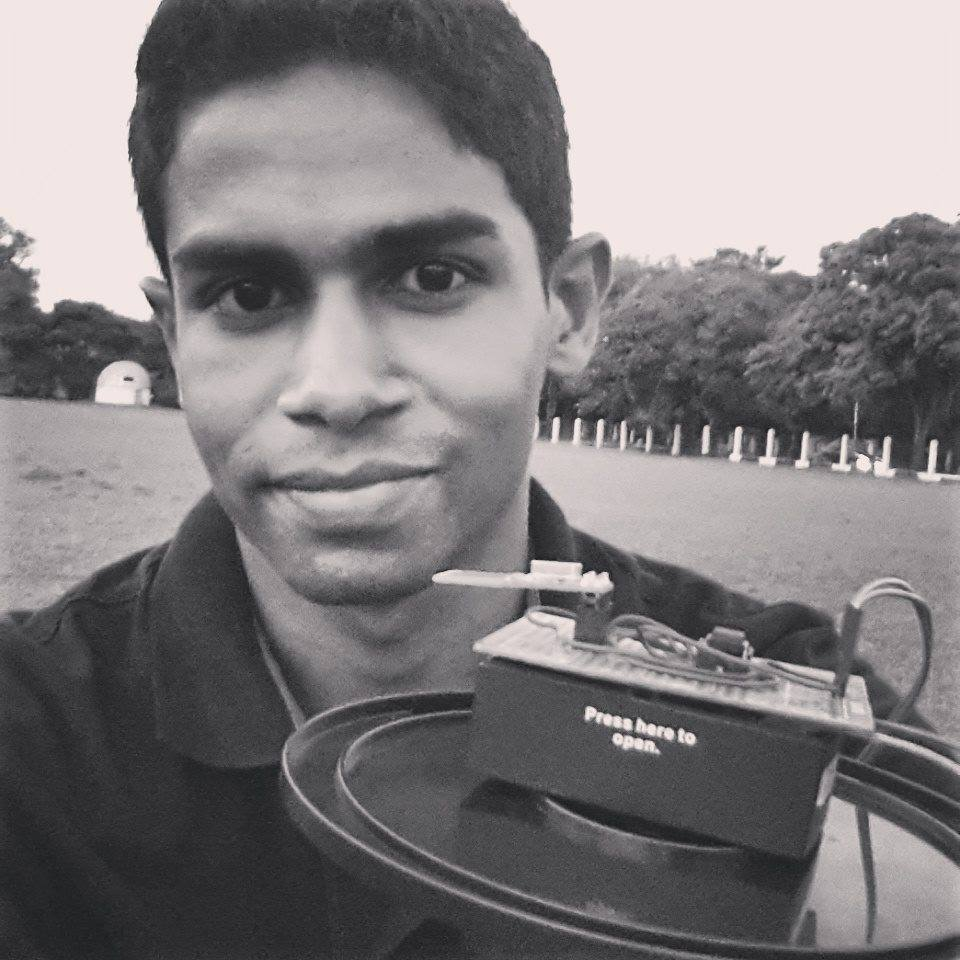
\includegraphics[width=80pt]{figures/me-with-mote.jpg}
	\end{figure}

	\begin{itemize}
	\footnotesize
	\item Introduction to Computing (FoS), Digital Forensics, Embedded Systems, and Operating Systems II.
	\vspace{10pt}
	\item Running \emph{Signal Insights} research lab.
	\vspace{10pt}
	\item {\scriptsize \url{https://ucsc.cmb.ac.lk/profile/asa} \\ \url{https://www.asayakkara.org}}
	\end{itemize}

	\end{columns}
\end{frame}
%-------------------------------------------------------------------------------


%-------------------------------------------------------------------------------
\begin{frame}{Signal Insights Research Lab}  

	\begin{figure}
		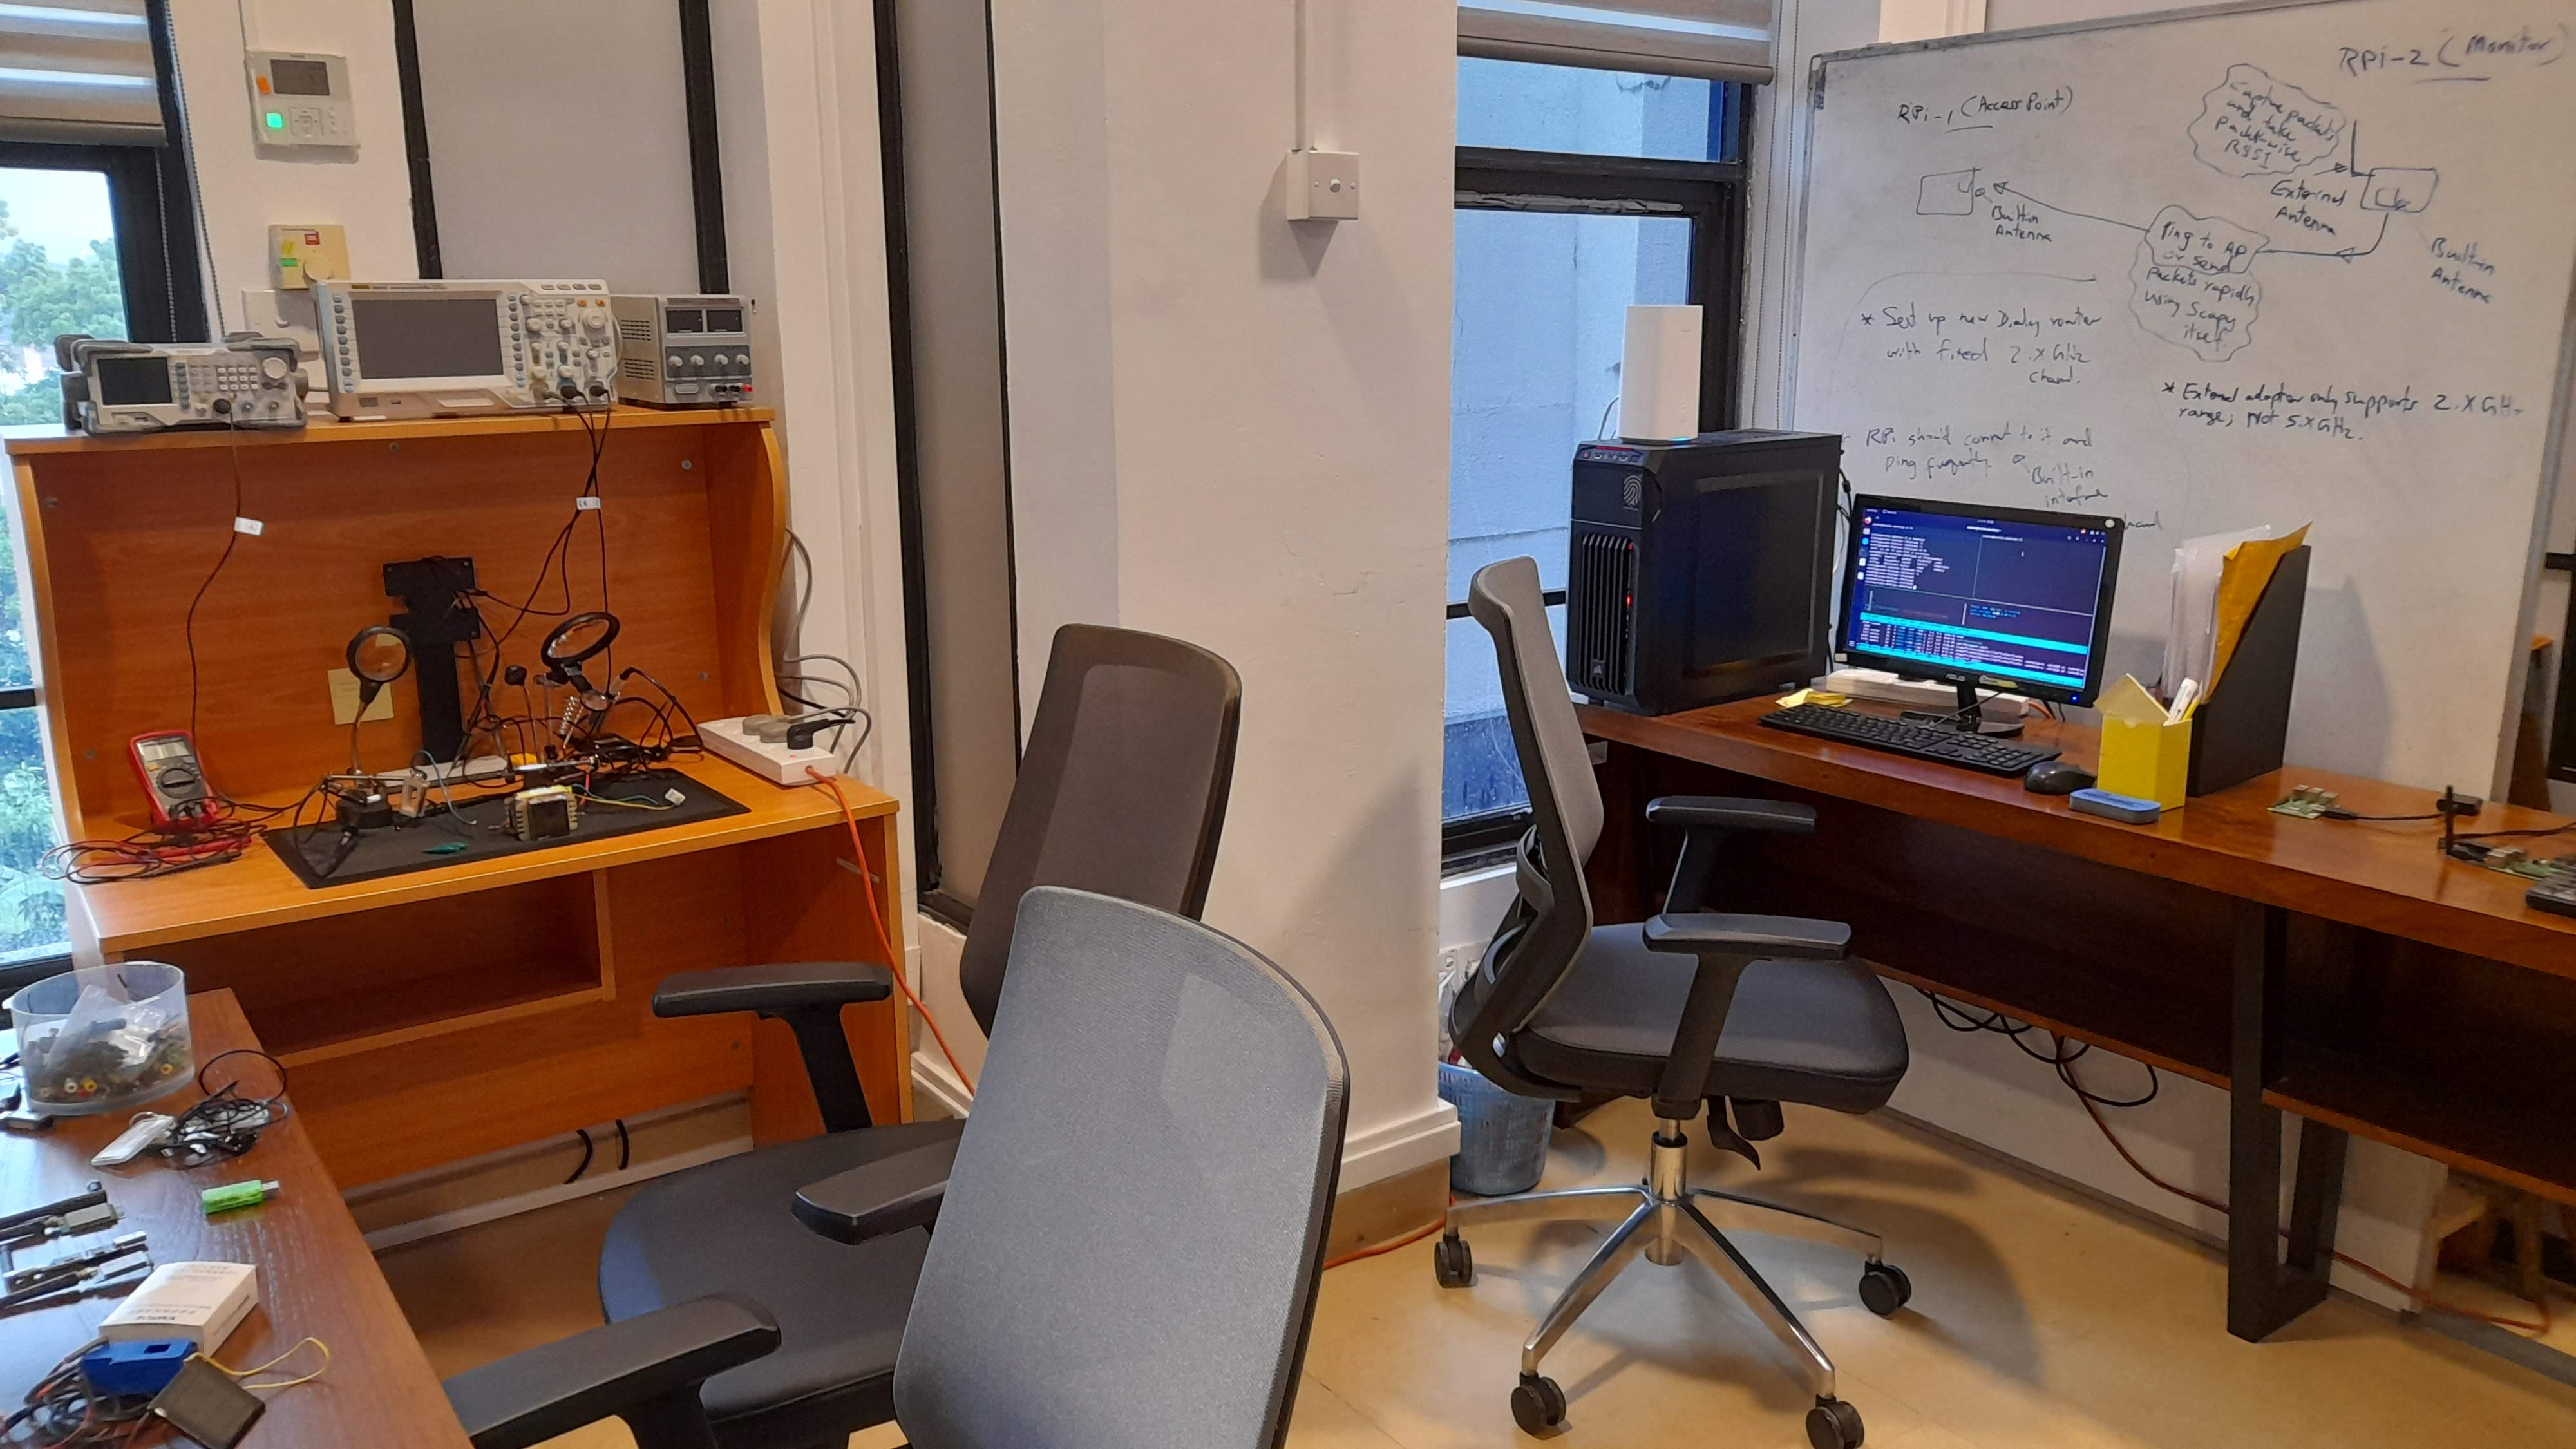
\includegraphics[width=180pt]{figures/signal-insights-lab-view.jpg}
	\end{figure}
	
	\begin{itemize}
		\footnotesize
		\item Explore the potential of exploiting various kinds of signals originating from various sources.  
		\item Signal sources: artificial, as well as biological sources (bioacoustics).
		\item Electromagnetic side-channels and covert channels.
		\item Radio tomographic imaging.
		\item Passive acoustic monitoring (of elephants).
		\item {\scriptsize \url{https://www.asayakkara.org/signal-insights-lab.html}}
	\end{itemize}

\end{frame}
%-------------------------------------------------------------------------------


%-------------------------------------------------------------------------------
\begin{frame}{Workshop Agenda}  

	\begin{itemize}
	\footnotesize
	\item \textbf{Part 1:}
		\begin{itemize}
		\footnotesize
		\item Introduction and background
		\item SDR hardware.
		\item SDR software.
		\item Capturing EM side-channel radiation.
		\end{itemize}
		\vspace{10pt}
	\item[] Break
		\vspace{10pt}
	\item \textbf{Part 2:}
		\begin{itemize}
		\footnotesize
		\item Analysing EM datasets using Python.
		\item Build your own Arduino program classifier.
		\item Discussion and conclusion
		\end{itemize}
	\end{itemize}

\end{frame}
%-------------------------------------------------------------------------------


%-------------------------------------------------------------------------------
\begin{frame}{}  

	\begin{block}{Introduction and Background}
	\end{block}

\end{frame}
%-------------------------------------------------------------------------------


%-------------------------------------------------------------------------------
\begin{frame}{Challenge of IoT \& Smart Device Forensics}  

	\begin{figure}
		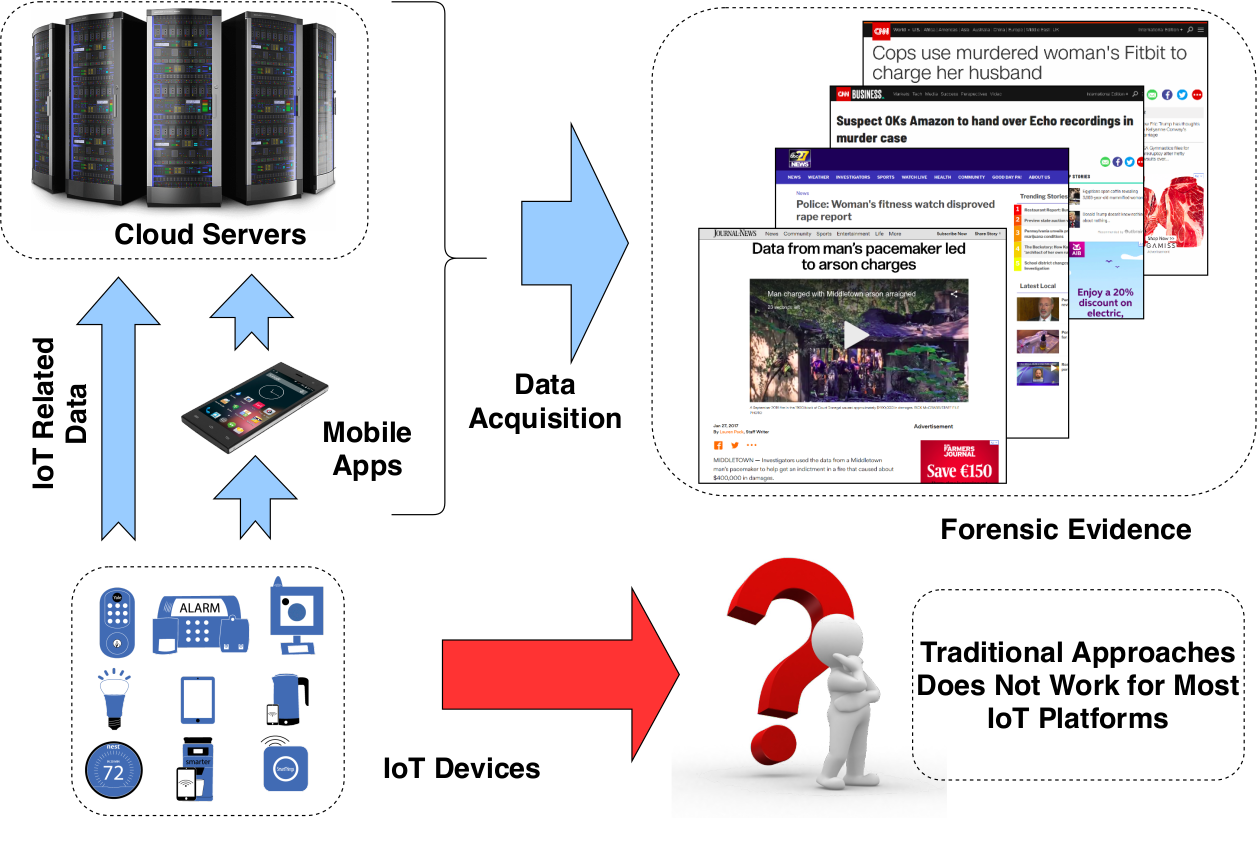
\includegraphics[width=250pt]{figures/IoT-forensic-challenge-small.png}
	\end{figure}

\end{frame}
%-------------------------------------------------------------------------------


%-------------------------------------------------------------------------------
\begin{frame}{Challenge of IoT \& Smart Device Forensics (cont.)}  

\begin{itemize}
\footnotesize
\item New devices are emerging in the market too frequently.
\vspace{10pt}
\item The internal components, storage, and interfaces of the devices varies drastically.
\vspace{10pt}
\item Analysing devices at too close to the hardware level --- such as chip-off forensics --- is susceptibe to irreversible mistakes that can destroy a device entirely.
\vspace{10pt}
\item It would be ideal if we can inspect a device from a safe distance.
\end{itemize}

\end{frame}
%-------------------------------------------------------------------------------



%-------------------------------------------------------------------------------
\begin{frame}{Evidence vs Insights}  

\begin{columns}

	\column{0.4\textwidth}

	\begin{figure}
		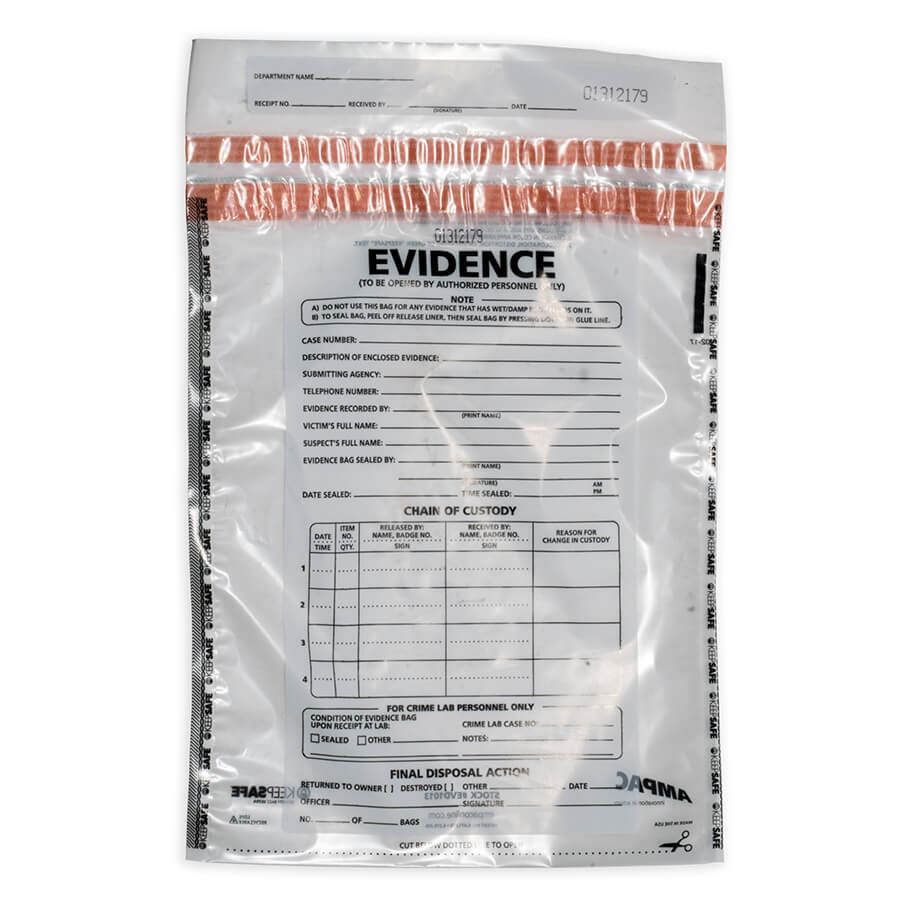
\includegraphics[width=150pt]{figures/digital-evidence.jpg}
	\end{figure}

	\column{0.6\textwidth}

	\begin{itemize}
	\footnotesize
	\item Digital \textbf{evidence} are information that may be presented to a court of law.
		\vspace{10pt}
	\item They need to be concrete enough to be relied upon at the courts.
		\vspace{10pt}
	\item The field of digital forensics is aimed at providing this reliability as much as possibile.
		\vspace{10pt}
	\item In some situations, where evidence are not available, some \textbf{insights} can a lifeline for an investigator. 
		\vspace{10pt}
	\item Insights are --- most likely --- not reproducible, but they can provide useful hints and directions to go and locate reliable evidence through other means. 
	\end{itemize}

\end{columns}

\end{frame}
%-------------------------------------------------------------------------------


%-------------------------------------------------------------------------------
\begin{frame}{Forensic Insights from IoT and Smart Devices}  

	\begin{itemize}
	\footnotesize
	\item Is this device running the official firmware from the manufacturer?
		\vspace{10pt}
	\item Has a malware been injected to the memory of this device?
		\vspace{10pt}
	\item Is this device doing something it is not supposed to be doing right now; such as wiping the storage or encrypting it, instead of shutting down?
	\end{itemize}

\end{frame}
%-------------------------------------------------------------------------------


%-------------------------------------------------------------------------------
\begin{frame}{Electromagnetic Side-Channel Analysis}  

	\begin{itemize}
	\footnotesize
	\item Time-varying electrical currents are generating electromagnetic (EM) radiation.
		\vspace{10pt}
	\item Our electronic equipment are a source of strong EM radiation.
		\vspace{10pt}
	\item The EM radiation of computers (specifically, the processors) is shown to be correlating with the software running on them, i.e., the exact instructions and their execution pattern.
		\vspace{10pt}
	\item EM Side-Channel Analysis (EM-SCA) is the exploitation of these radiation to eavesdrop on computers:
		\vspace{5pt}
		\begin{itemize}
		\footnotesize
		\item Software behaviour dection.
		\vspace{10pt}
		\item Malicious firmware modification detection.
		\vspace{10pt}
		\item Cryptographic key retrieval.
		\end{itemize}
	\end{itemize}

\end{frame}
%-------------------------------------------------------------------------------


%-------------------------------------------------------------------------------
\begin{frame}{Electromagnetic Side-Channel Analysis (cont.)}  

\footnotesize
A Few Demonstrations
\vspace{10pt}

\begin{itemize}
	\footnotesize
	\item Radiation from the laptop screen/graphic card:\\ \url{https://www.youtube.com/watch?v=YtolwTPDBwk}
	\vspace{10pt}
	\item Remote servelliance of video displays:\\ \url{http://www.youtube.com/watch?v=8OlkywZBJGU}
	\vspace{10pt}
	\item Data exfiltration through EM covert channel on an Ethernet cable:\\ \url{https://www.youtube.com/watch?v=ciM4M5h3q0w}
\end{itemize}

\end{frame}
%-------------------------------------------------------------------------------


%-------------------------------------------------------------------------------
\begin{frame}{Forensic Insights through EM-SCA}  

	\begin{figure}
		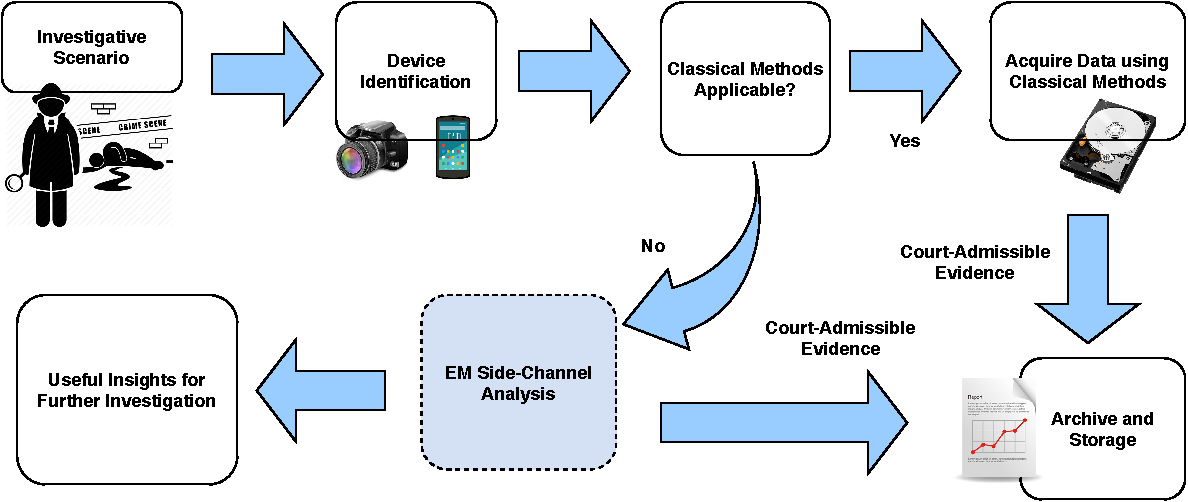
\includegraphics[width=280pt]{figures/applying-em-sca-to-forensic-process.pdf}
	\end{figure}

\end{frame}
%-------------------------------------------------------------------------------



%-------------------------------------------------------------------------------
\begin{frame}{}  

	\begin{block}{Software Defined Radios}
	\end{block}

\end{frame}
%-------------------------------------------------------------------------------


%-------------------------------------------------------------------------------
\begin{frame}{Software Defined Radios}  

\begin{itemize}
	\footnotesize
	\item Moving most of radio functions from analog domain into the digital domain.
	\vspace{10pt}
	\item Requires a generic hardware radio interface including a very fast analog-to-digital converter (ADC).
	\vspace{10pt}
	\item Need sophisticated and optimised software implementations for digital signal processing (DSP).
\end{itemize}

	\begin{figure}
		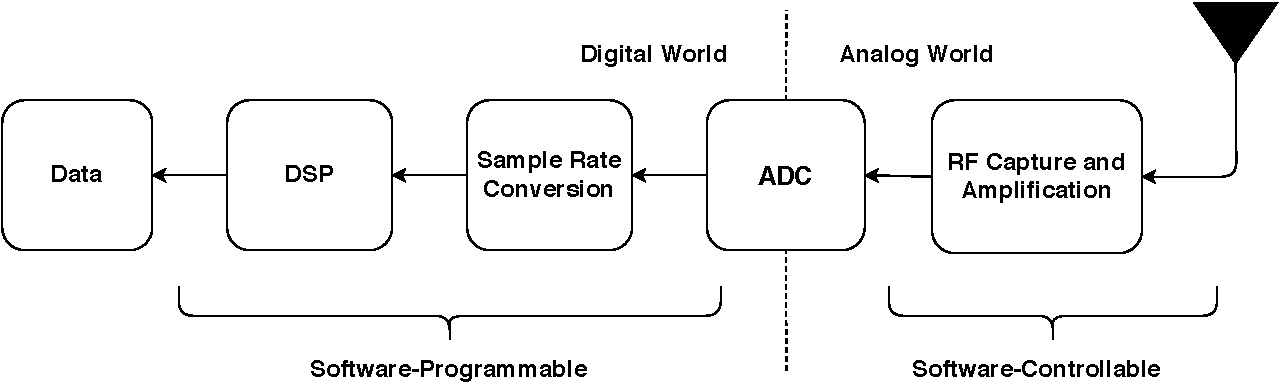
\includegraphics[width=290pt]{figures/sdr-architecture.pdf}
	\end{figure}

\end{frame}
%-------------------------------------------------------------------------------


%-------------------------------------------------------------------------------
\begin{frame}{Software Defined Radios (cont.)}  

	\footnotesize
	Converting analog signals to digital signals require \textbf{sampling} and \textbf{quantisation}. 

	\begin{figure}
		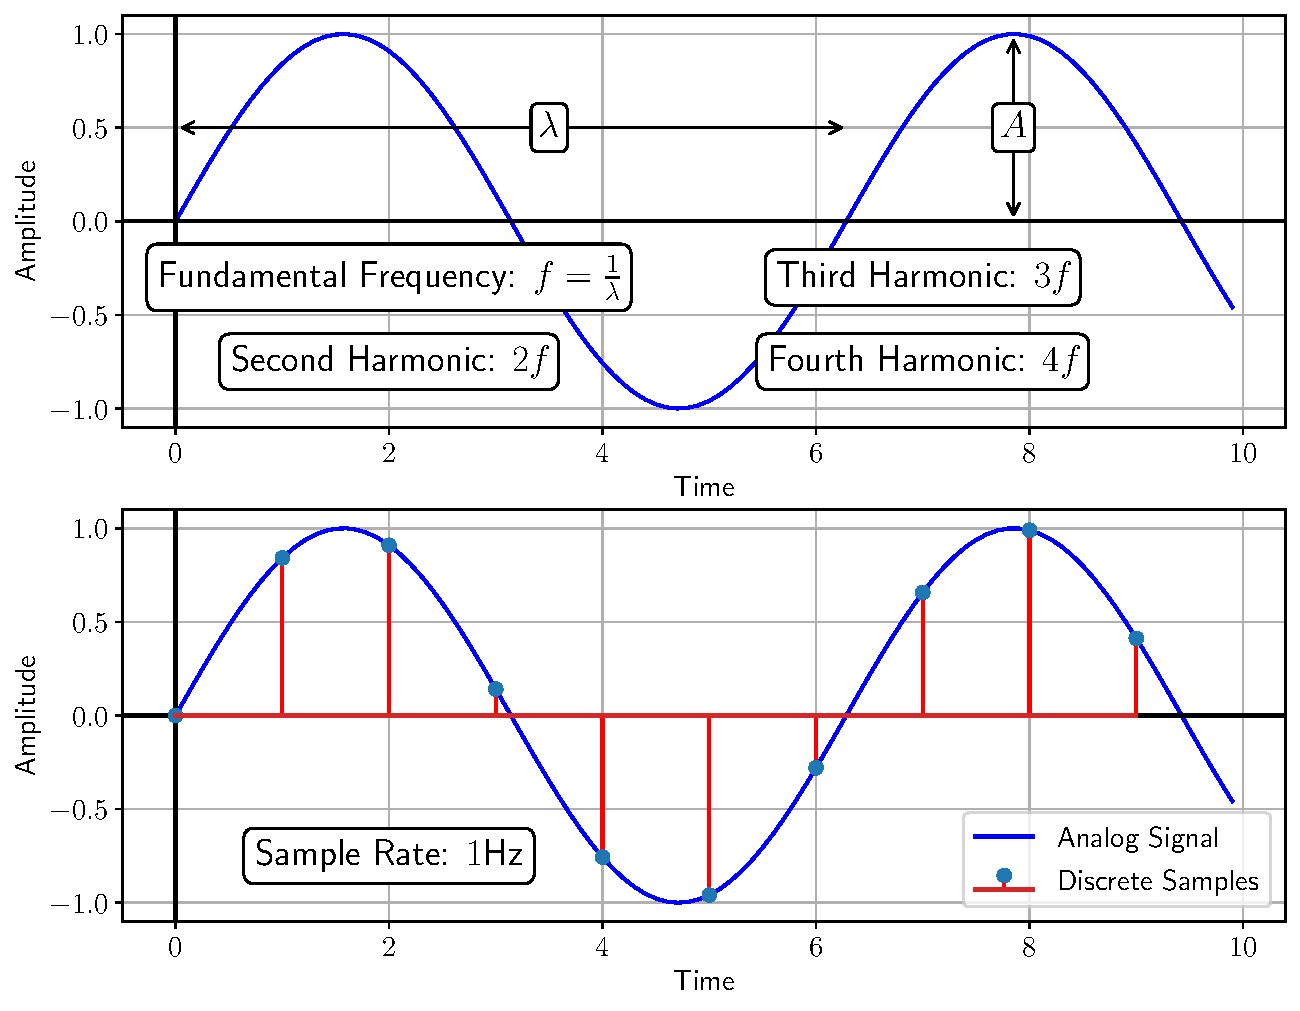
\includegraphics[width=210pt]{figures/signal-properties.pdf}
	\end{figure}

	\footnotesize
	\textbf{Real-valued sampling} faces the Nyquist limit: difficult to capture high frequencies.

\end{frame}
%-------------------------------------------------------------------------------


%-------------------------------------------------------------------------------
\begin{frame}{Software Defined Radios (cont.)}  

	\begin{itemize}
	\footnotesize
	\item SDRs are using complex \textbf{In-phase/Quadrature-phase (I/Q)} sampling.
		\vspace{5pt}
	\item Each sample taken at a given time instance consists of two values; hence, each sample is a complex number.
		\vspace{5pt}
	\item A EM signal captured by an SDR is basically an array of complex numbers.
		\vspace{5pt}
	\item Sampling rate is equal to the bandwidth of the captured data.
	\end{itemize}

	\begin{figure}
		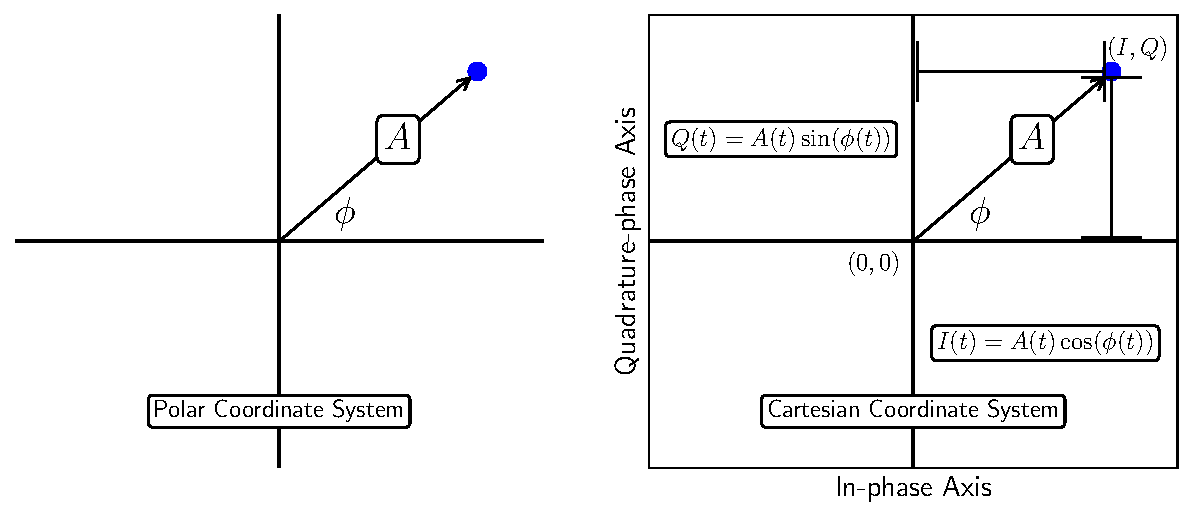
\includegraphics[width=280pt]{figures/iq-representation.pdf}
	\end{figure}

	\footnotesize

\end{frame}
%-------------------------------------------------------------------------------


%-------------------------------------------------------------------------------
\begin{frame}{Software Defined Radios (cont.)}  

\footnotesize
\textbf{RTL-SDR}

\begin{columns}

	\column{0.4\textwidth}

	\begin{figure}
		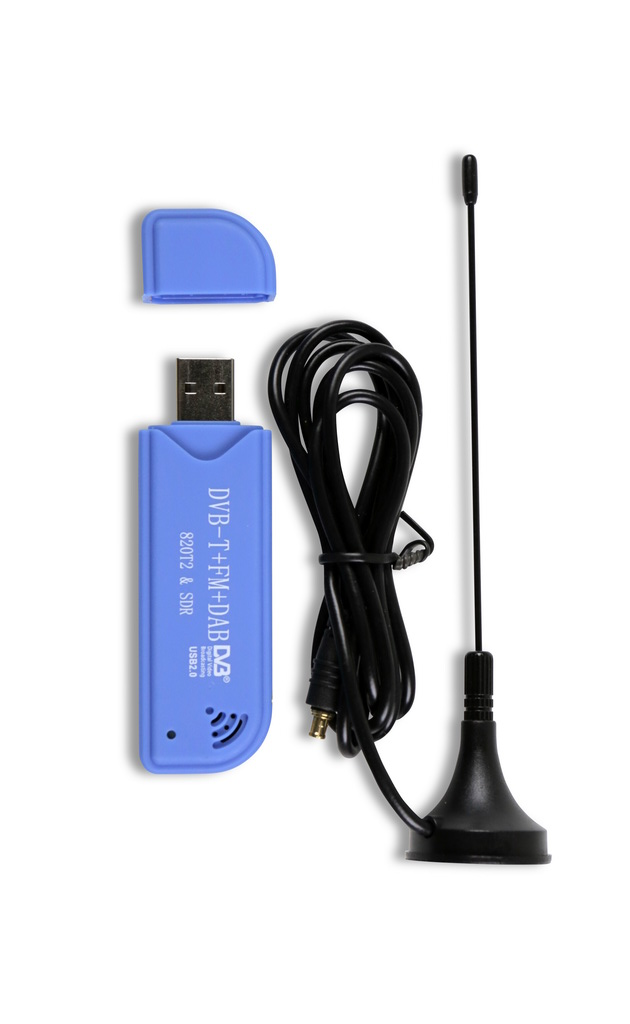
\includegraphics[width=100pt]{figures/rtl-sdr.jpg}
	\end{figure}

	\column{0.6\textwidth}

	\begin{itemize}
	\footnotesize
	\item A digital TV tuner repurposed as an SDR.
		\vspace{5pt}
	\item The cheapest possible SDR you may find.
		\vspace{5pt}
	\item A wide variety of manufacturers; hence different variations of capabilities.
		\vspace{5pt}
	\item Sample rate is about 3.2 MHz
		\vspace{5pt}
	\item Tunable frequency range: 22 MHz -- 1 GHz.
		\vspace{5pt}
	\item Receive only; no transmission.
	\end{itemize}


\end{columns}

\end{frame}
%-------------------------------------------------------------------------------


%-------------------------------------------------------------------------------
\begin{frame}{Software Defined Radios (cont.)}  

\footnotesize
\textbf{HackRF One}

\begin{columns}

	\column{0.4\textwidth}

	\begin{figure}
		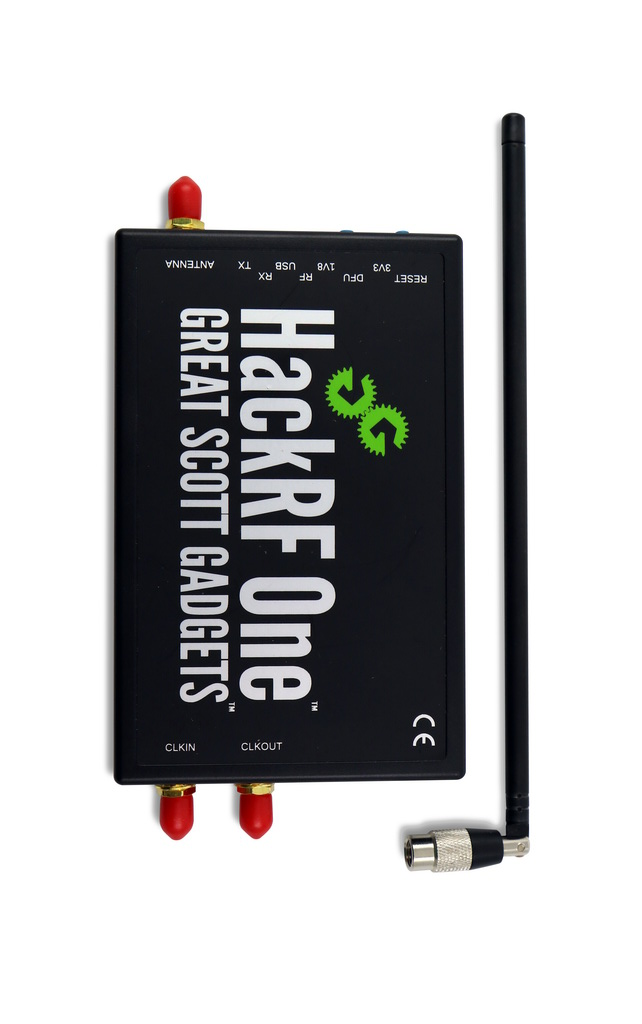
\includegraphics[width=120pt]{figures/hackrf-one.jpg}
	\end{figure}

	\column{0.6\textwidth}

	\begin{itemize}
	\footnotesize
	\item A purpose-built SDR device.
		\vspace{5pt}
	\item A mid-range price tag.
		\vspace{5pt}
	\item Sample rate: upto 20 MHz.
		\vspace{5pt}
	\item Tunable frequency range: 1 MHz -- 6 GHz.
		\vspace{5pt}
	\item A wide range of antennas can be connect through the SMA connector.
		\vspace{5pt}
	\item Half-duplex: either transmit or receive at a given time.
		\vspace{5pt}
	\item Possible to time-synchronise with another device through clock input or output.
	\end{itemize}


\end{columns}

\end{frame}
%-------------------------------------------------------------------------------


%-------------------------------------------------------------------------------
\begin{frame}{Software Defined Radios (cont.)}  

\footnotesize
\textbf{GQRX}

	\begin{itemize}
	\footnotesize
	\item Easily view signals at different frequencies.
		\vspace{5pt}
	\item Facilitates live processing and saving observed signals.
		\vspace{5pt}
	\item Uses \emph{GNURadio} library underneath.
	\end{itemize}

	\begin{figure}
		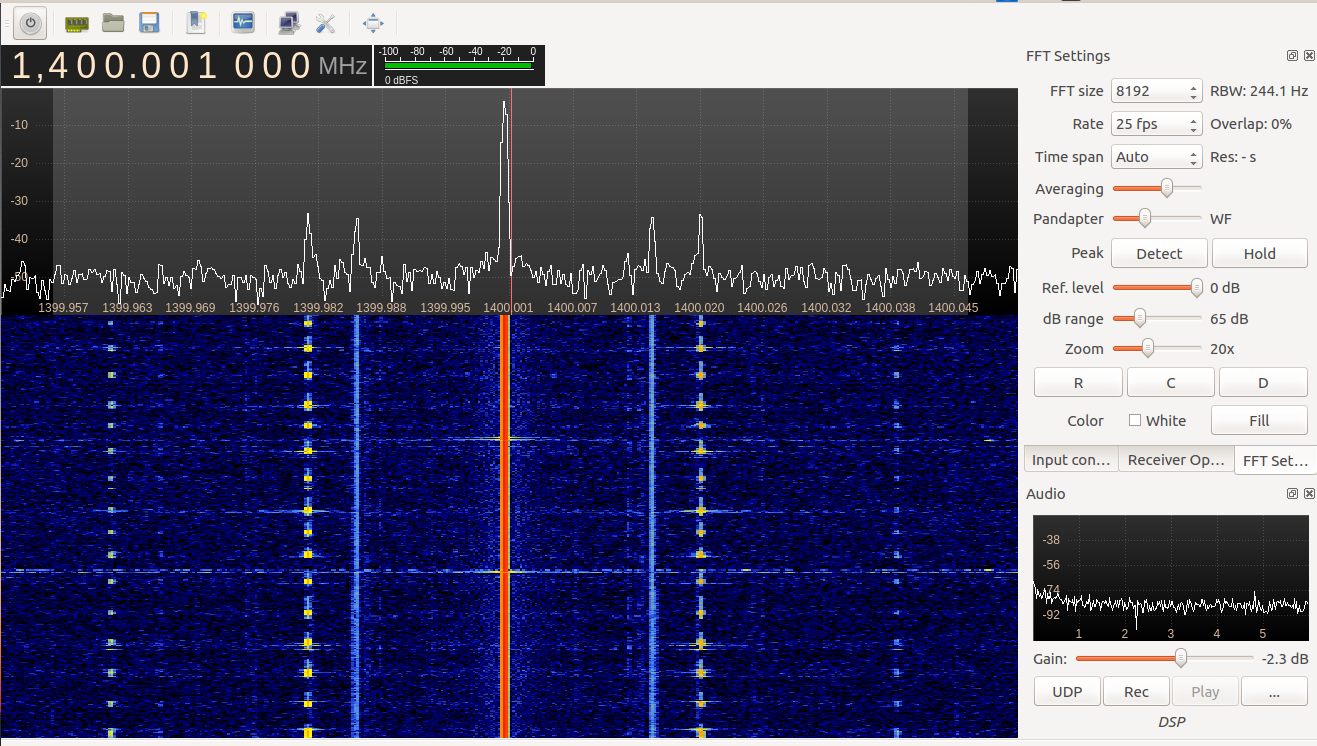
\includegraphics[width=200pt]{figures/gqrx-window.png}
	\end{figure}

\end{frame}
%-------------------------------------------------------------------------------


%-------------------------------------------------------------------------------
\begin{frame}{Software Defined Radios (cont.)}  

\footnotesize
\textbf{GNURadio Companion (GRC)}

	\begin{itemize}
	\footnotesize
	\item Various signal processing blocks.
		\vspace{5pt}
	\item Custom build any application by creating flow graph using blocks.
		\vspace{5pt}
	\item Generates executable Python scripts for flow graphs, using \emph{GNURadio} library.
	\end{itemize}

	\begin{figure}
		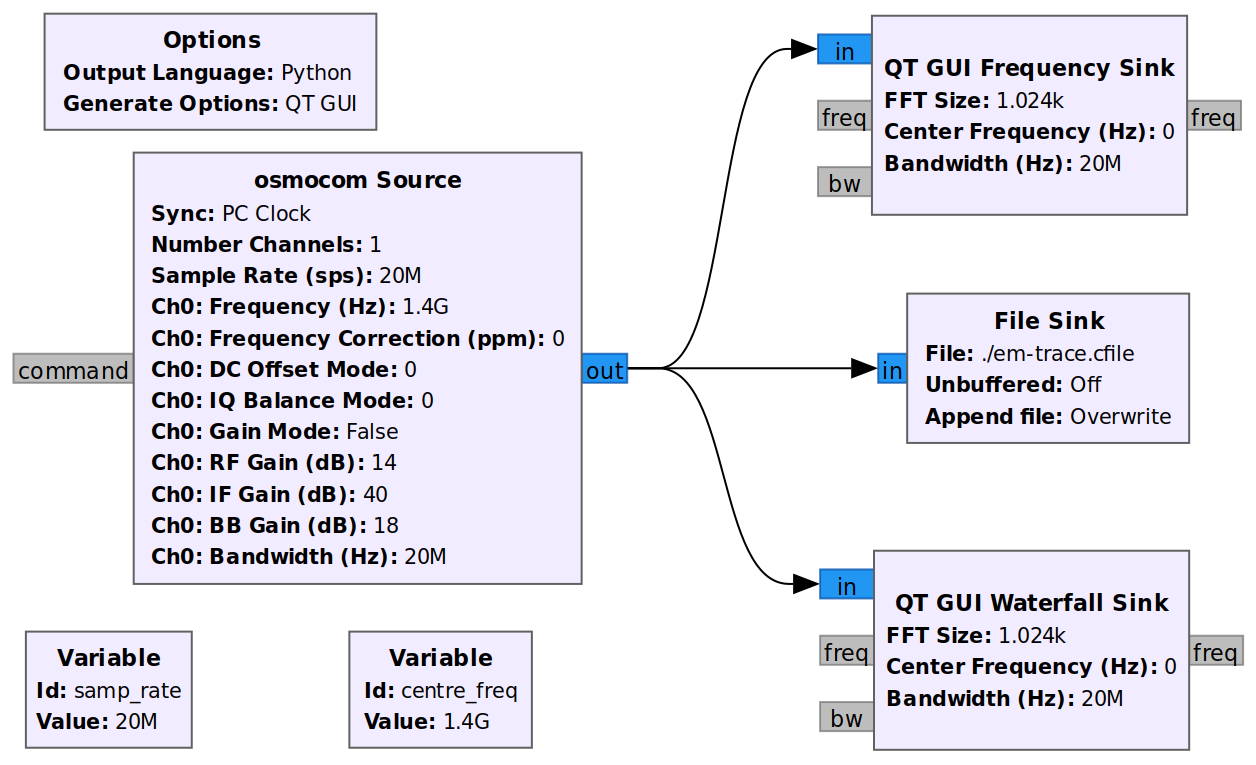
\includegraphics[width=200pt]{figures/grc-flowgraph-for-data-acquisition.png}
	\end{figure}

\end{frame}
%-------------------------------------------------------------------------------


%-------------------------------------------------------------------------------
\begin{frame}{}  

	\begin{block}{Capturing EM Side-Channel Radiation}
	\end{block}

\end{frame}
%-------------------------------------------------------------------------------


%-------------------------------------------------------------------------------
\begin{frame}{Capturing EM Side-Channel Radiation}  

	\begin{itemize}
	\footnotesize
	\item Our key focus is EM radiation from the processor/microcontroller/SoC.
		\vspace{5pt}
	\item Strongest signals are in the clock frequency or its harmonics.
		\vspace{5pt}
	\item Signal acquisition should be performed as closer to the target chip as possible.
		\vspace{5pt}
	\item Magnetic H-loop antennas are more suitable for the job.
	\end{itemize}


	\begin{figure}
		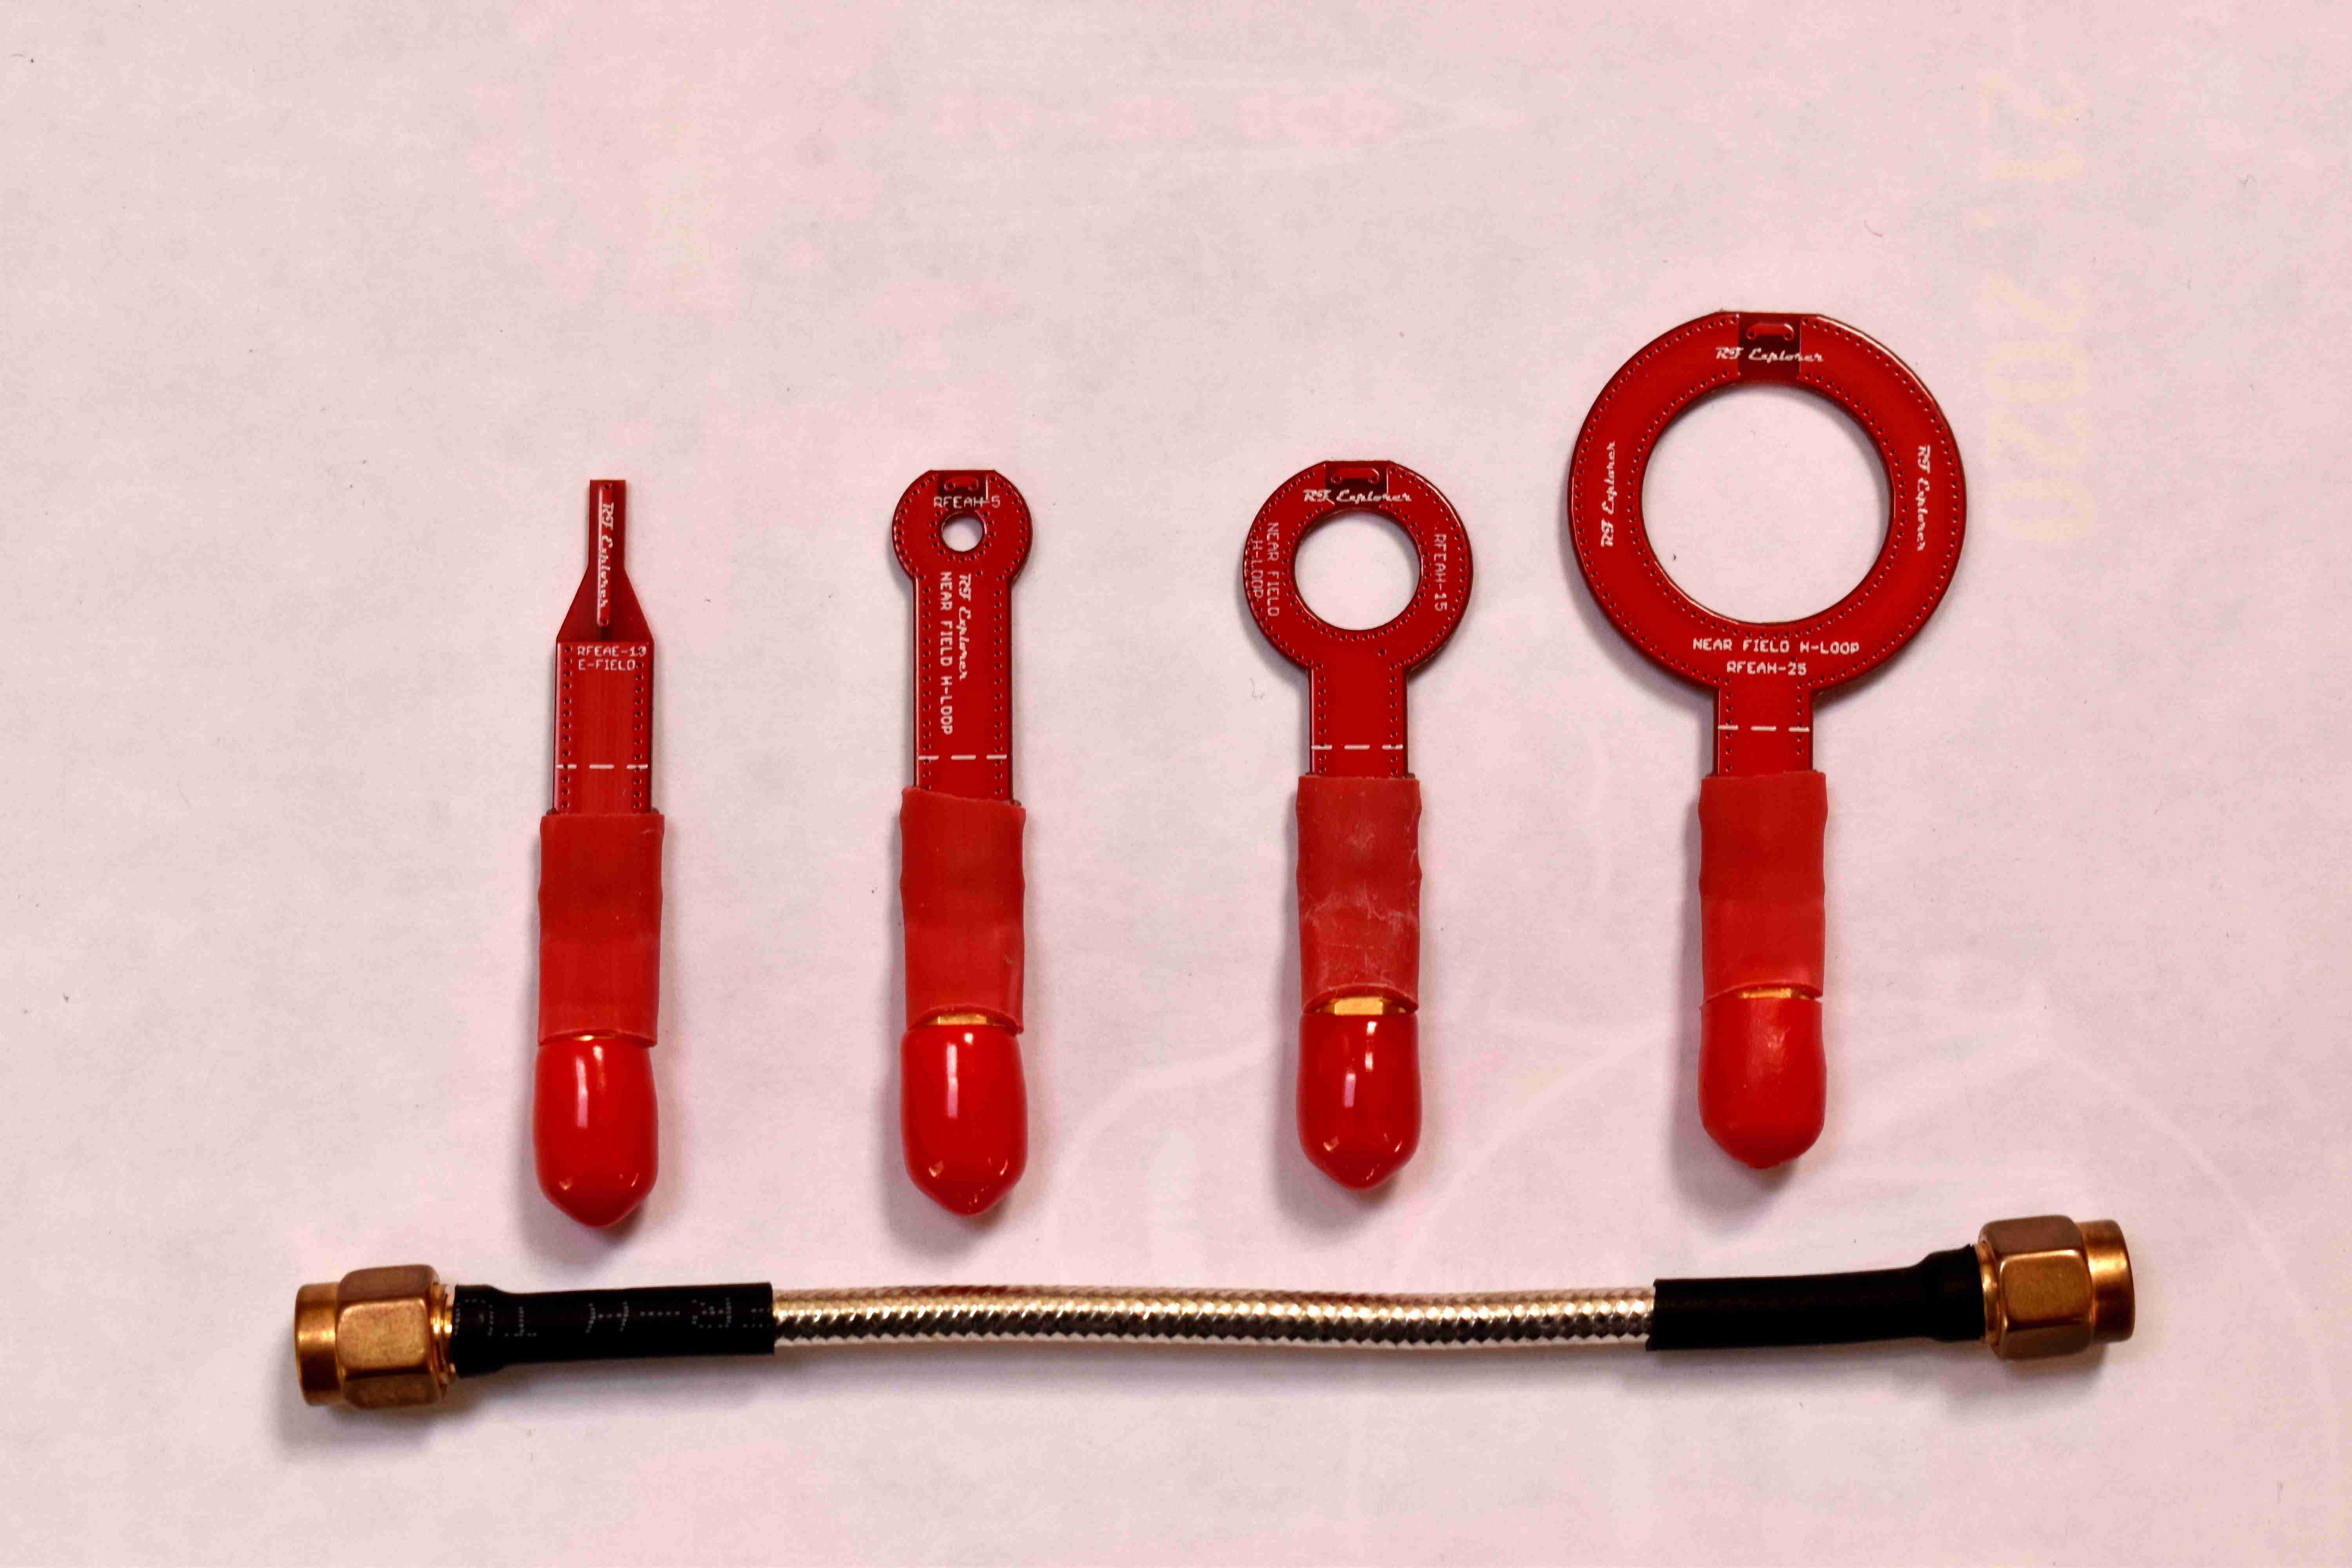
\includegraphics[width=140pt]{figures/antenna-kit-small.jpg}
	\end{figure}

\end{frame}
%-------------------------------------------------------------------------------



%-------------------------------------------------------------------------------
\begin{frame}{Capturing EM Side-Channel Radiation (cont.)}  

\footnotesize
\textbf{Passive acquisition:}

	\begin{figure}
		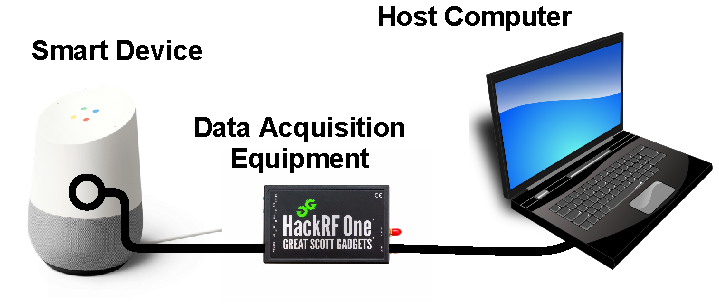
\includegraphics[width=210pt]{figures/hardware-setup.pdf}
	\end{figure}

\end{frame}
%-------------------------------------------------------------------------------


%-------------------------------------------------------------------------------
\begin{frame}{Capturing EM Side-Channel Radiation (cont.)}  

\footnotesize
\textbf{Instrumented acquisition:}

	\begin{figure}
		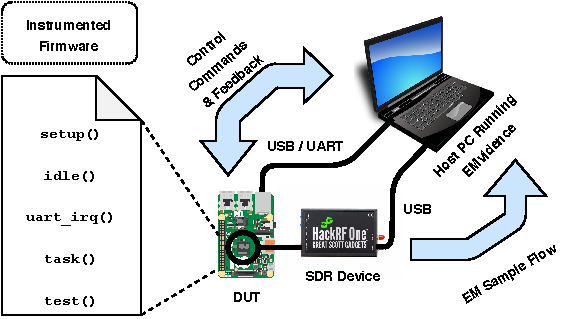
\includegraphics[width=210pt]{figures/signal-acquisition-2.pdf}
	\end{figure}

\end{frame}
%-------------------------------------------------------------------------------


%-------------------------------------------------------------------------------
\begin{frame}{Capturing EM Side-Channel Radiation (cont.)}  

\footnotesize
\textbf{Arduino and Raspberry Pi}

	\begin{figure}
		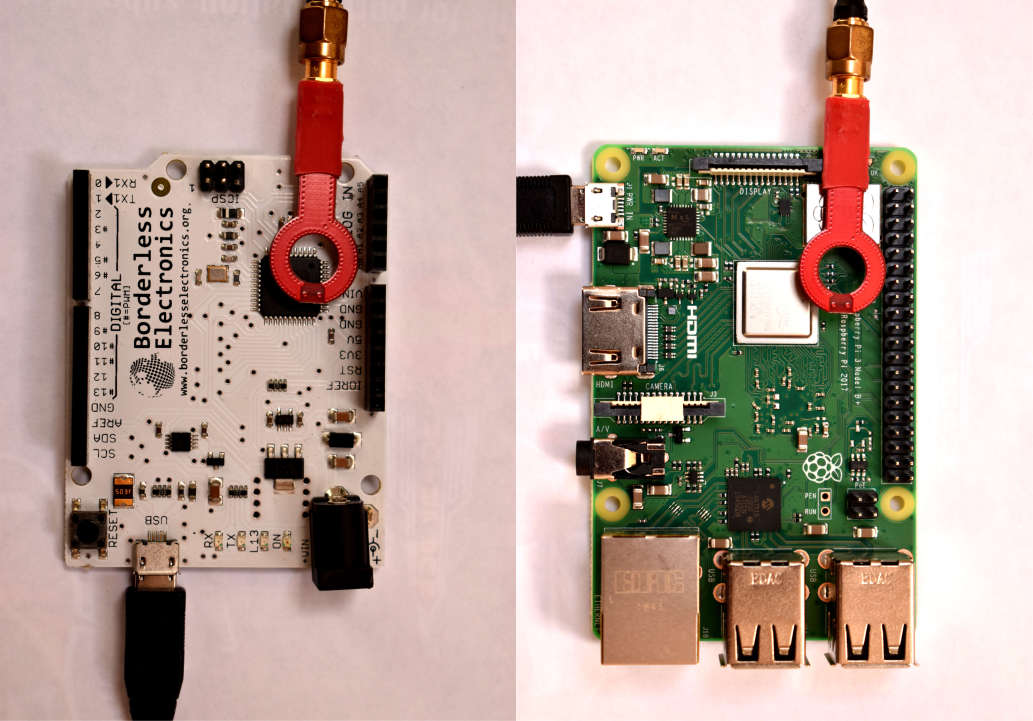
\includegraphics[width=200pt]{figures/arduino-rpi-with-antenna.jpg}
	\end{figure}

\end{frame}
%-------------------------------------------------------------------------------


%-------------------------------------------------------------------------------
\begin{frame}{Capturing EM Side-Channel Radiation (cont.)}  

\footnotesize
\textbf{Smartphone}

	\begin{figure}
		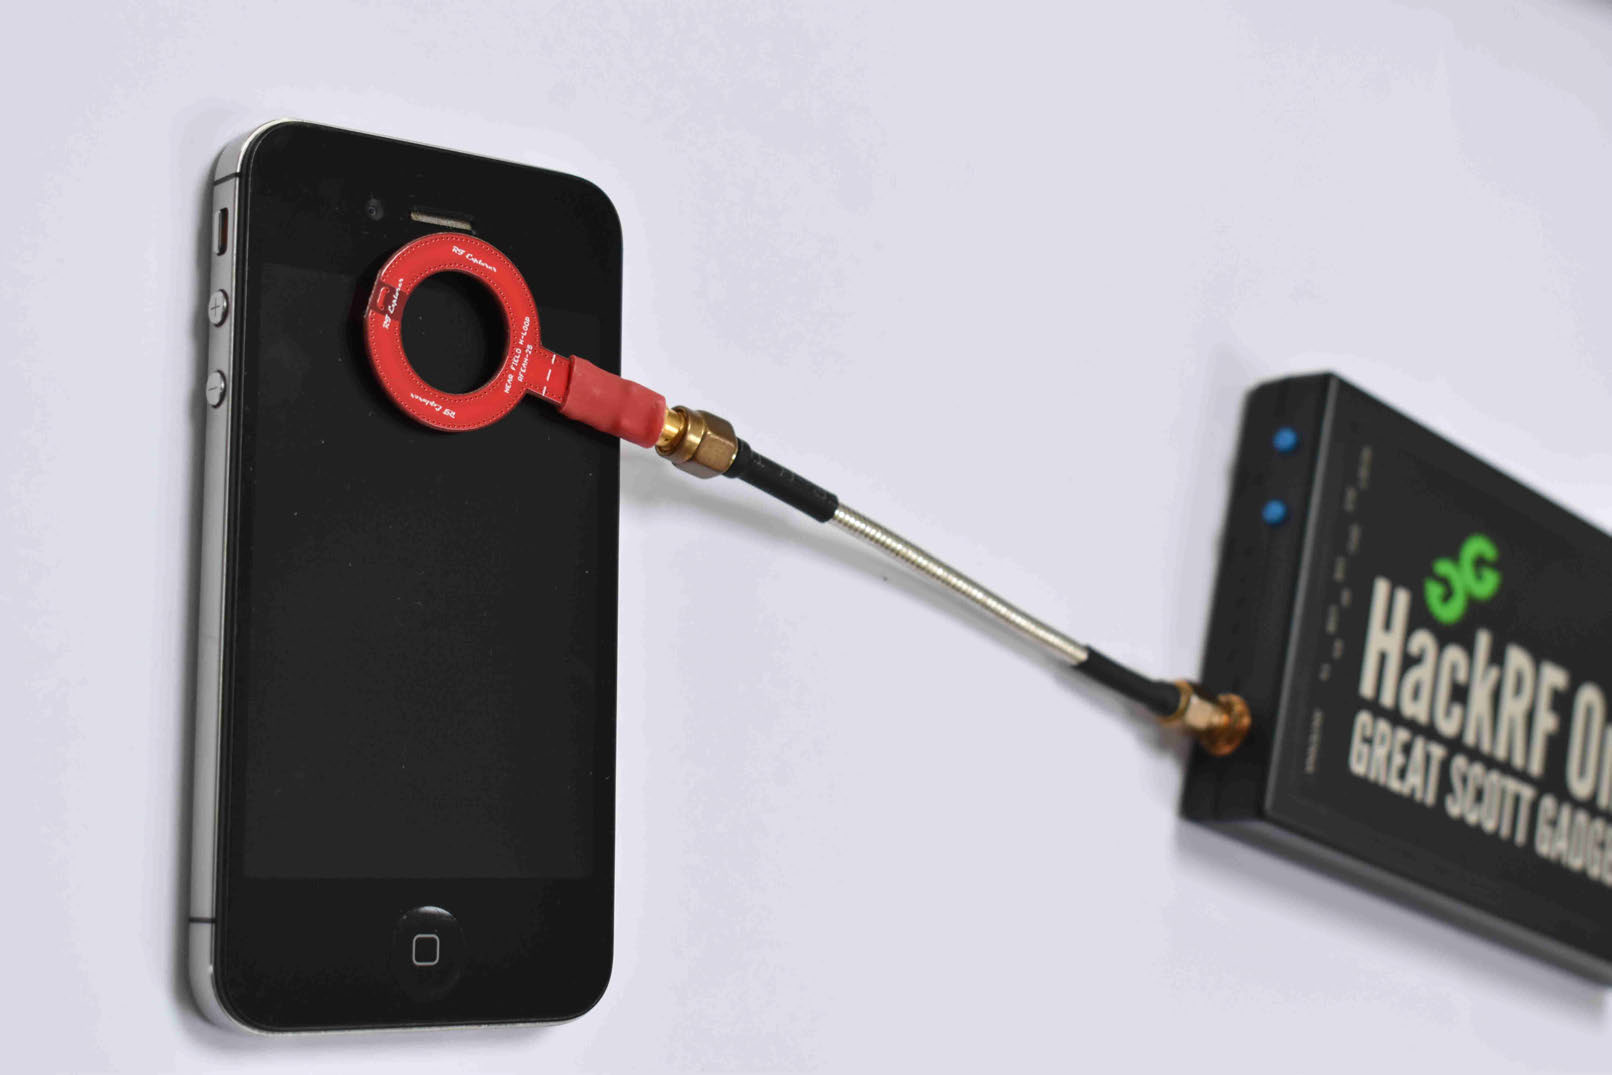
\includegraphics[width=200pt]{figures/iphone-hackrf.png}
	\end{figure}

\end{frame}
%-------------------------------------------------------------------------------



%-------------------------------------------------------------------------------
\begin{frame}{}  

	\begin{block}{Analysing EM Dataset}
	\end{block}

\end{frame}
%-------------------------------------------------------------------------------

%-------------------------------------------------------------------------------
\begin{frame}{Analysing EM Dataset}  

\footnotesize
The pipeline from capturing EM data to analysis...

	\begin{figure}
		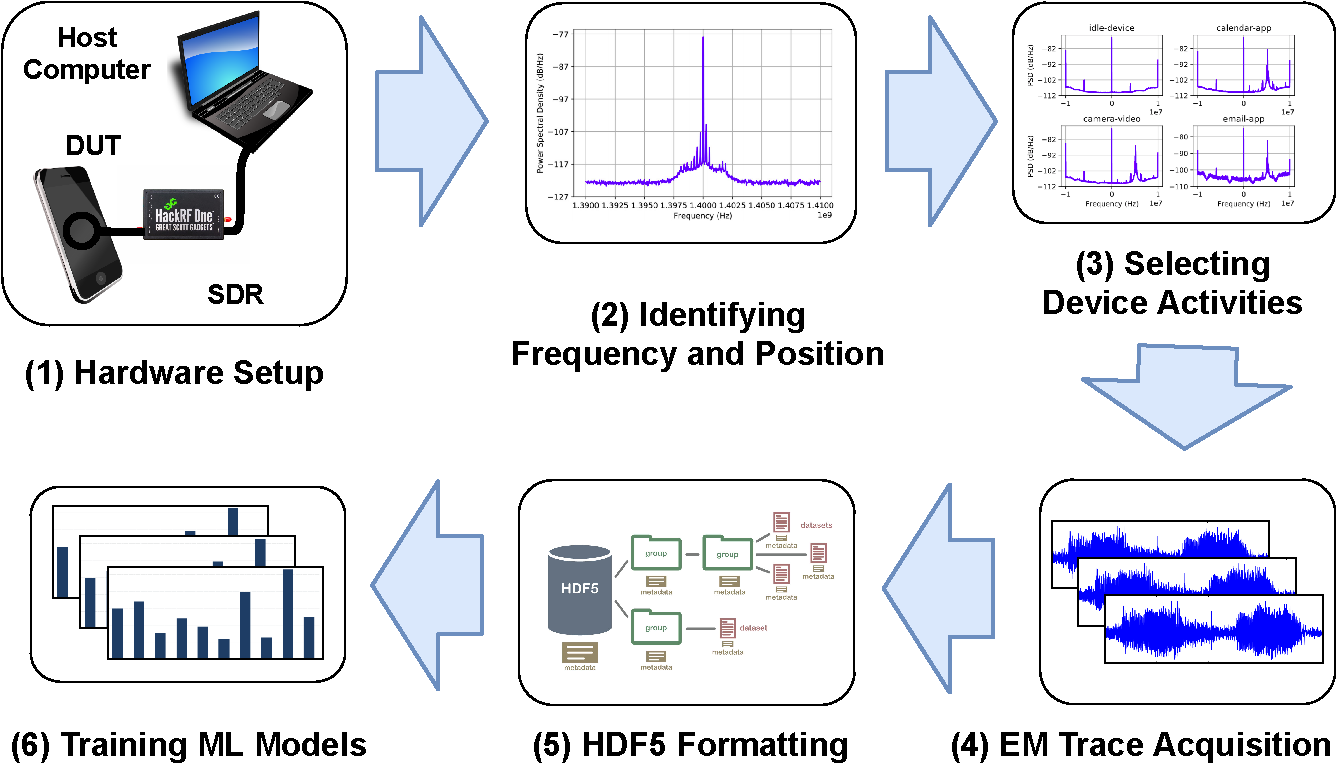
\includegraphics[width=230pt]{figures/sdr-data-pipeline-V2.pdf}
	\end{figure}

\end{frame}
%----------------------------------------------------------------------


%-------------------------------------------------------------------------------
\begin{frame}{Analysing EM Dataset}  

\footnotesize
\textbf{Huge Size of the Data Files}
		\vspace{10pt}

	\begin{itemize}
	\item In GNU Radio library, two 32 bit (4 byte) floating point values are used to represent a complex I/Q sample.
		\vspace{10pt}
	\item Therefore, each EM data sample is a 8 bytes long complex value.
		\vspace{10pt}
	\item Consider if we sampled data at the maximum sample rate of HackRF One device (i.e., 20 MHz) using GNURadio library to save data.
		\vspace{10pt}
	\item Size of data per second = $8$ bytes $\times 20 \times 10^{6} = 160$ MB
		\vspace{10pt}
	\item Size of data for 10 seconds = $160$ MB $\times 10 = 1.6$ GB
	\end{itemize}

\end{frame}
%----------------------------------------------------------------------


%-------------------------------------------------------------------------------
\begin{frame}{Analysing EM Dataset (cont.)}  

\footnotesize
The specifications of devices in the dataset:
	

	\begin{figure}
		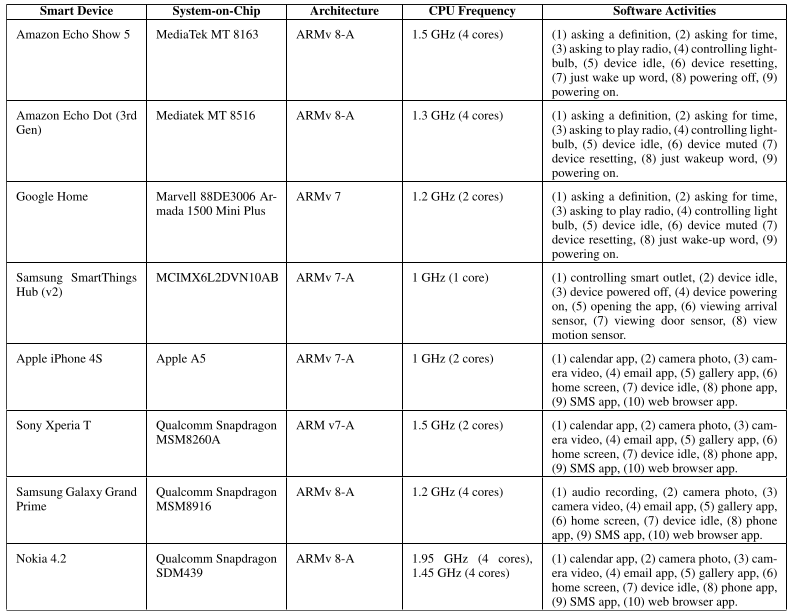
\includegraphics[width=250pt]{figures/device-spec-from-the-dataset.png}
	\end{figure}

\end{frame}
%--------------------------------------


%-------------------------------------------------------------------------------
\begin{frame}{Analysing EM Dataset (cont.)}  

	\footnotesize
	Structure of the dataset in HDF5 file format (em-dataset.h5):

	\begin{figure}
		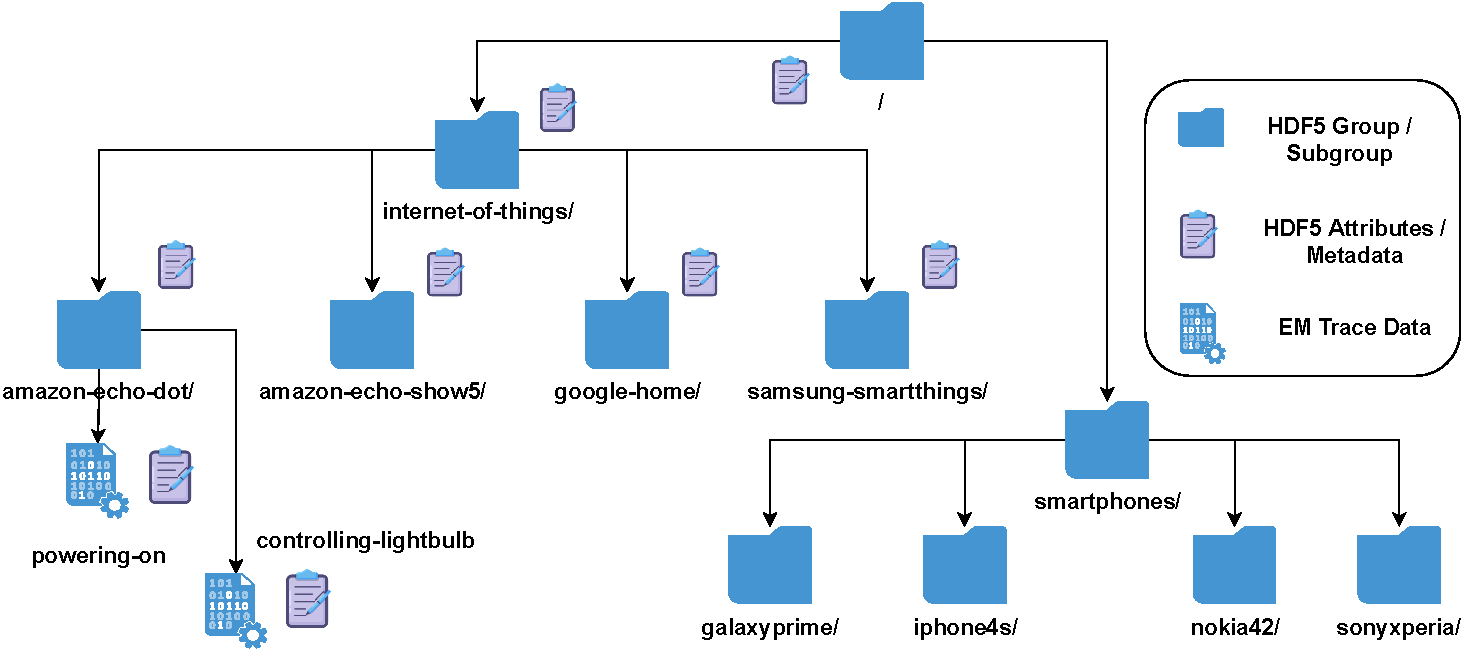
\includegraphics[width=280pt]{figures/hdf5-dataset-structure.pdf}
	\end{figure}

\end{frame}
%--------------------------------------

%-------------------------------------------------------------------------------
\begin{frame}{Analysing EM Dataset (cont.)}  

	\footnotesize
	Amazon Echo Dot -- Power Spectral Density (PSD) Plots

	\begin{figure}
		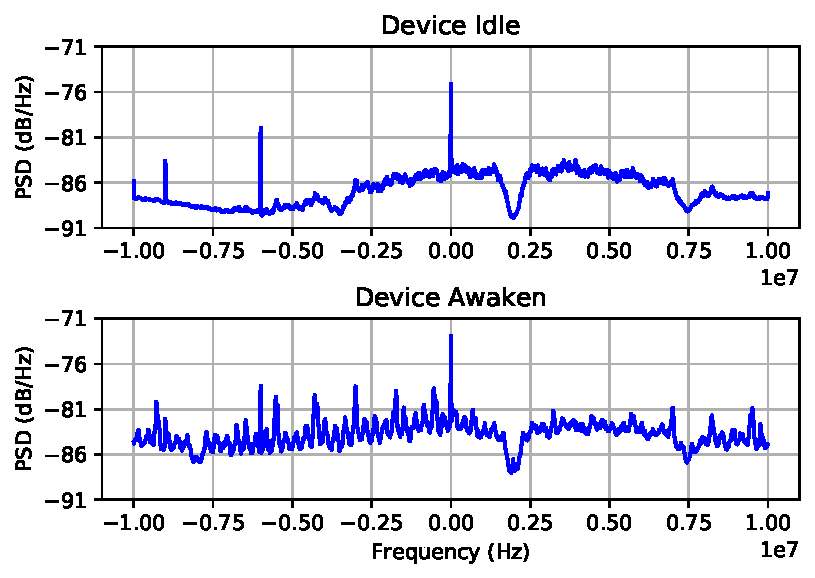
\includegraphics[width=240pt]{figures/amazon-echo-dot-psd-plots.pdf}
	\end{figure}

\end{frame}
%--------------------------------------


%-------------------------------------------------------------------------------
\begin{frame}{Analysing EM Dataset (cont.)}  

	\footnotesize
	Nokia 4.2 -- Histogram

	\begin{figure}
		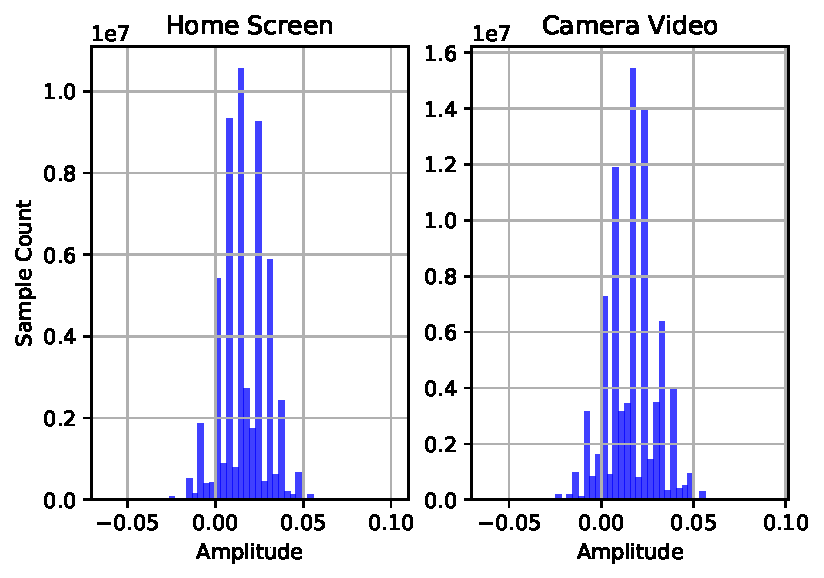
\includegraphics[width=240pt]{figures/data-distribution-plots-Nokia42.pdf}
	\end{figure}

\end{frame}
%--------------------------------------


%-------------------------------------------------------------------------------
\begin{frame}{Analysing EM Dataset (cont.)}  

	\begin{itemize}
	\footnotesize
	\item Go ahead and launch Jupyter Notebook inside the downloaded Git repository.
		\vspace{10pt}
	\item We'll explore the code examples for the following things:
		\vspace{10pt}
		\begin{enumerate}
		\footnotesize
		\item Reading and basic visualisation of EM data.
		\vspace{5pt}
		\item Preprocessing EM data for feature extraction.
		\vspace{5pt}
		\item Simple machine learning classifiers to distinguish software behaviour.
		\end{enumerate}
	\end{itemize}

\end{frame}
%-------------------------------------------------------------------------------


%-------------------------------------------------------------------------------
\begin{frame}{Build Your Arduino Classifier}

\begin{itemize}
\footnotesize
\item Shall we collect our own data and build a classifier for software behaviour detection?
\vspace{10pt}
\item We can program an Arduino Uno to do two different tasks and capture two EM data files representing each task.
\vspace{10pt}
\item Let's see if we can build a simple classifier to distinguish between the two tasks.
\end{itemize}

\end{frame}
%-------------------------------------------------------------------------------


%-------------------------------------------------------------------------------
\begin{frame}{Conclusion}

\begin{itemize}
\footnotesize
\item EM-SCA for digital forensic insight acquisition is still in its early days.
\vspace{10pt}
\item Loads of technical and scientific problems remaining to be solves; great for research!
\vspace{10pt}
\item \emph{Cross-device portability} of trained models.
\vspace{10pt}
\item No need to possess hardware equipment to conduct research in this area; datasets are available to work on (from our group and many others).
\vspace{10pt}
\item Thank you for your participation. Feel free to get in touch: \\ 
	\vspace{5pt} 
	Asanka Sayakkara (\texttt{asa@ucsc.cmb.ac.lk})
\end{itemize}

\end{frame}
%-------------------------------------------------------------------------------


%-------------------------------------------------------------------------------
\begin{frame}{References}

\begin{enumerate}
\scriptsize
\item Asanka Sayakkara, Le-Khac, N-A., and Scanlon, M., ``Electromagnetic Side-Channel Attacks: Potential for Progressing Hindered Digital Forensic Analysis", International Workshop on Speculative Side Channel Analysis (WoSSCA 2018), Amsterdam, Netherlands, July 2018.
\vspace{10pt}
\item Asanka Sayakkara, Le-Khac, N-A., and Scanlon, M., ``A Survey of Electromagnetic Side-Channel Attacks and Discussion on their Case-Progressing Potential for Digital Forensics", Elsevier Digital Investigation, 2019. 
\vspace{10pt}
\item Asanka Sayakkara, Le-Khac, N-A., and Scanlon, M., ``Leveraging Electromagnetic Side-Channel Analysis for the Investigation of IoT Devices", DFRWS USA, Portland, OR, USA, July 2019.
\vspace{10pt}
\item Asanka Sayakkara and Nhien-An Le-Khac , ``Electromagnetic Side-Channel Analysis for IoT Forensics: Challenges, Framework, and Datasets," in IEEE Access, vol 9, pp. 113585-113598, 2021. 
\vspace{10pt}
\item[] Find more here: \url{https://www.asayakkara.org/publications.html}
\end{enumerate}

\end{frame}
%-------------------------------------------------------------------------------



\end{document}


